\section{Background} \label{sec:background}
\subsection{Evolutionary Algorithms}
At the genesis of modern computing, the 1950s, researchers began to apply advancing computational capabilities to investigate and test models of biological evolution. Very quickly they realized the potential of virtual evolution to achieve other ends, setting into motion a line of research that has since blossomed into the field of evolutionary algorithms (EA) design. These algorithms, which use mechanics inspired by biological evolution to evolve novel solutions to a wide array of problems, share a generally consistent basic methodology. The process begins with a population of randomly generated solutions. In a generation-based loop, an elite subset of the population is selected for their fitness (their quality as a solution), subjected to random changes, and recombined with each other to form the next generation. The cycle repeats for as many iterations as desired, and fitness tends to increase with each iteration. Figure \ref{fig:working_principle} provides a graphical overview of this process.
\begin{figure}
\centering
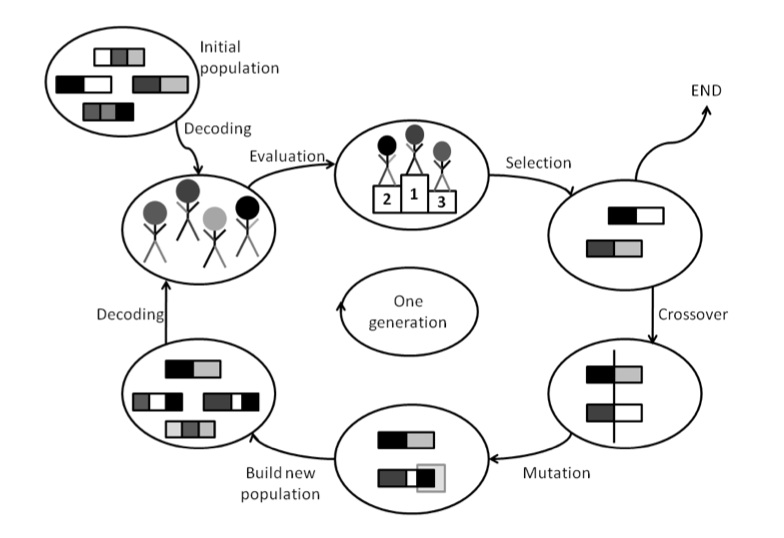
\includegraphics[width=0.5\textwidth]{img/working_principle_of_EA.jpg}
\caption{\label{fig:working_principle} Evolutionary algorithms traditionally operate in a generation-based loop that, over the course of many iterations, gradually refines a population of candidate solutions, which is initialized with randomly-generated individuals, to generate increasingly fit individuals. That is, individuals that provide an increasingly satisfactory solution to a particular problem. At the start of each cycle of the loop, individual solutions are generated from a population of genotypes. These solutions are scored by a fitness function, which measures the performance of the individual as a solution to the problem. Then, the genetic material of fit individuals are mutated and recombined to create the next generation of candidate individuals. Once a predefined stopping criterion is met, usually a maximum number of generations or threshold fitness score, the evolutionary cycle is halted \cite{Prothmann2009EvolutionaryOptimisation}}.
\end{figure}


Researchers and engineers have widely demonstrated the ability of EA to attack labor-intensive optimization problems and to discover novel solutions beyond the reach of human ingenuity \cite{Poli2008AProgramming}. The intervening half century of EA research has seen diversification of the general evolutionary search process described above and diversification of the contents and format of candidate solutions. Solutions can be a set of real values, such as the component dimensions of a satellite truss optimized to minimize vibration resistance. Solutions can also be represented as branched connections between operations and values, colloquially known as a ‘tree.’ This type of EA is known as genetic programming (GP). Essentially, candidate solutions in traditional GP are mathematical expressions formatted for flexibility in recombination and manageability of expression in code. \cite{Poli2008AProgramming}. A distinction can also be drawn between mutation-based approaches such as evolution strategies or evolutionary programming and crossover-based approaches, which rely on a distinct theory based around the concept of schemata, the collections of fixed points on chromosomal bitstrings that, as a unit, confer fitness to an individual \cite{2006RepresentationsAlgorithms}. In practice, however, a combination of crossover and mutation, to generate background noise to the process, is typically favored, such as the standard simple genetic algorithm (GA).

\subsection{Neural Networks}

Artificial neural networks, as mentioned in Section \ref{sec:motivation}, have rapidly cemented themselves as a cornerstone of modern computer science. These systems are loosely modeled on the distributed neural architecture of the brain. At the most basic level, neural networks can be described as a chain of weighted and re-scaled sums. These networks are traditionally organized into distinct, ordered layers of nodes, with each layer determining its values based on those of the previous layer and the first and last representing input and output, respectively, of the network. This scheme is called ``feed-forward'' because information flows from one layer to the next and out of the system, and is not retained in the system through cyclic topologies. A prototypical feed-forward network is illustrated in Figure \ref{fig:feed_forward}.

Networks are typically initiated with random or uniform initial connectivity weightings, which are refined through an iterative trial-and-error-driven process known as training where the network is adjusted towards exhibiting a desired behavior. Consider, for illustration, a network intended to identify images that contained cats. To train the network, a set of training data consisting of images labeled for whether or not they depict a cat would be necessary. The network would be exposed to one image at a time; this input would be processed by the network, in this case producing a single output -- whether or not the network thinks the image contains a cat. If the network's output deviates from the desired output, the weights of connections between neurons in the network are slightly adjusted through backpropagation, which essentially calculates which connection weights were to blame for the improper output and adjusts those connections in the direction of the error function's steepest descent. After exposure to many training cases and adjustments to the network to minimize overfitting to the training data, the resulting network will more reliably identify images that contain cats (even in images that it was not trained on).

Recent advances in the field have been made by employing back-propagation with deep neural networks (networks with many hidden layers between the input and output layers). While this method is both powerful and computationally tractable, it has significant limitations including the necessity of supervised learning during the training process (each training input must be coupled with a known, desired output), poor ability to train networks with recurrence (i.e. networks with memory), the possibility of getting stuck at local maxima, and lack of network adaptability post-training \cite[pg 312, 364]{Downing2015IntelligenceSystems}. 
\begin{figure}
\centering
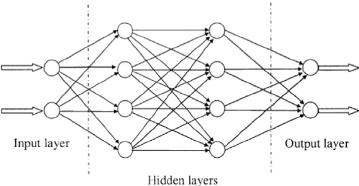
\includegraphics[width=0.6\textwidth]{img/Fig-1-Schematic-diagram-of-a-multilayer-feed-forward-neural-network-3.png}
\caption{\label{fig:feed_forward} An illustration of a feed-forward neural network with two hidden layers \cite{Griffiths2015IntroductionAnalysis}} 
\end{figure}

\subsection{Glossary}

This section reviews a handful of terms that are essential to discussions of evolution and evolutionary algorithms.

\subsubsection{Individual}

Individual are the object upon which evolution operates; evolution evaluates and selects on individuals and recombines individuals to form new individuals. In biology, and individual is an individual organism such as a single tree or a single bird. In evolutionary algorithms, an individual is abstracted as a candidate solution to a problem.

\subsubsection{Population}

A population is a collection of individuals that compete to transmit their genetic information to the next generation. These individuals are typically highly similar and, in many cases in both biology and evolutionary algorithms, recombine their genetic information to produce offspring.

\subsubsection{Phenotype}

Phenotype refers to the characteristics of an individual that interact with its environment to determine its fitness. In biology, the physical form of an organism (i.e. its body) is the phenotype. In evolutionary algorithms, the phenotype refers to the characteristics of an individual that are evaluated during selection.

\subsubsection{Genotype}

Genotype refers to information that is used to determine the phenotype that is passed from generation to generation. In biology, a DNA sequence serves as the genotype. Although many different genotypic encodings are employed in evolutionary algorithms, in evolutionary algorithms the genotype ultimately boils down to a collection of digital information.

\subsubsection{Recombination}

Recombination refers to the generation of new genetic material from existing genetic material. This can involve combinations of two or more sets of genetic material, as in sexual reproduction, and/or random perturbation of genetic information (i.e. mutations).

\subsubsection{Selection}

Selection refers to the determination of which individuals will pass genetic material on to the next generation by creating offspring (and how many offspring they will be able to generate) and which will not.

\subsubsection{Fitness}

Fitness refers to the success of an individual at passing its genetic information to the next generation. An individual with high fitness creates many offspring while an individual with low fitness does not. Success at surviving challenges posed by the environment is an important factor in determining fitness. In evolutionary algorithms, the concept of fitness is abstracted to the fitness function where an individual is scored based on its aptitude at performing a certain task.